\documentclass[11pt, oneside]{article}   	% use "amsart" instead of "article" for AMSLaTeX format
\usepackage{geometry}                		% See geometry.pdf to learn the layout options. There are lots.
\geometry{letterpaper}                   		% ... or a4paper or a5paper or ... 
%\geometry{landscape}                		% Activate for for rotated page geometry
%\usepackage[parfill]{parskip}    		% Activate to begin paragraphs with an empty line rather than an indent
\usepackage{graphicx}				% Use pdf, png, jpg, or eps� with pdflatex; use eps in DVI mode
								% TeX will automatically convert eps --> pdf in pdflatex		
\usepackage{amssymb}
\usepackage{amsmath}
\usepackage{parskip}
\usepackage{color}

\title{Newton to Kepler}
%\author{The Author}
%\section{}
% \subsection*{R code}
\date{}							% Activate to display a given date or no date

\graphicspath{{/Users/telliott_admin/Dropbox/Tex/png/}}

% \begin{center} 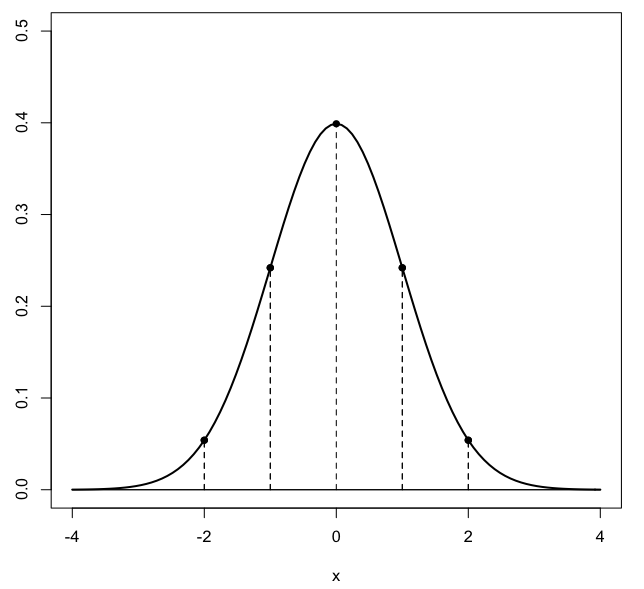
\includegraphics [scale=0.4] {gauss3.png} \end{center}

\begin{document}
\maketitle
\Large
\noindent
\begin{center} 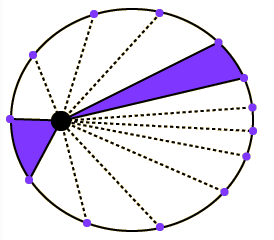
\includegraphics [scale=0.6] {equal_areas.png} \end{center}
I want to understand in detail how Kepler's Laws for the orbits of the planets can be derived from Newton's Laws, namely 

\[ \mathbf{F} = m \mathbf{a} \]

as well as the inverse square law of gravitation.  

\[ \mathbf{F} = -\frac{GMm}{r^2} \hat{\mathbf{u}}  \]

I've worked through derivations from several sources, and I think now that I have it figured out.  My goal is to clearly document things here so that I will understand in a year (or five) when I re-read this.

Kepler's Laws are:  first (K1), the orbits of the planets are not circles but ellipses (non-recurrent orbits may be other conic sections);  second (K2), the area or arc "swept out" per unit time is the same no matter where in the orbit the planet is;  and third (K3) the period of the orbit is independent of the mass of the planet and its square is proportional to the cube of the length of the semi-major axis of the ellipse.

I also spent some time working on Newton's version of the proof as presented in the \emph{Principia} (see Bressoud's vector calculus book), but he leaves out too many steps.  There is also a version "cooked up" by Richard Feynman and discussed in a book called \emph{Feynman's Lost Lecture}.  

I never got either of these figured out, but if you want to go this route I recommend starting with Feynman.

For myself, I found that once I cleared up a couple of subtleties,  and verified the application of the product rule for differentiation to vector cross-products, it was pretty easy.

\subsection*{circular approximation}
The equation of an ellipse in $xy$-coordinates is 
\[ \frac{x^2}{a^2} + \frac{y^2}{b^2} = 1 \]
where $a$ is one-half the "diameter" in the long dimension and $b$ is one-half the length perpendicular to that.

A second way is to give the focal length, the distance of each of the two foci from the center of the ellipse
\[ f = \sqrt{a^2 - b^2} \]
Yet another way is to give the \emph{eccentricity}, $e$, where 
\[ ea = f  \]
Here is a table of planetary eccentricities I found on the web.
\begin{center} 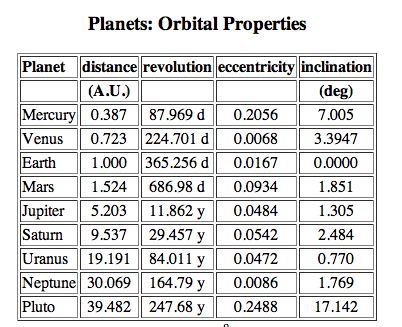
\includegraphics [scale=0.75] {eplanets.png} \end{center}
Mars is the planet that showed Kepler most clearly that the orbits are not circles, but its eccentricity is only 0.09.  For Earth this value is only $0.017$ which gives a focal length of roughly
\[ 0.0167 \times 149.6 \times 10^6 \ \text{km} \approx 2.5 \times 10^6 \ \text{km} \]
which is about four times the radius of the Sun.

However, there is a conflict with a simpler calculation, which I believe gives the correct answer, and I haven't figured that out yet.  The center of mass for the Sun-Earth system is (picking the center of the Sun as the origin)
\[ CM = \frac{M_E}{M_S} d_{ES} = \frac{6 \times 10^{24}}{2 \times 10^{30}} \ 1.5 \times 10^8 \ \text{km} = 450 \ \text{km} \]
compared to the radius of the Sun which is about $7 \times 10^5$ km.


\end{document}  